% !TeX spellcheck = en_GB
\documentclass[10pt,letterpaper,oneside]{article}
\usepackage{fontspec}
\usepackage{arev}
\usepackage[utf8]{inputenc}
\usepackage[T1]{fontenc}
\usepackage{amsmath}
\usepackage{amsfonts}
\usepackage{amssymb}
\usepackage{graphicx}
\usepackage{csquotes}
\usepackage{booktabs}
\usepackage{multicol}
\usepackage{enumerate}
\usepackage{microtype}
\usepackage[labelfont=bf,font={small}]{caption}
\usepackage{hyperref}
\usepackage{booktabs}
\usepackage{subcaption}
\usepackage{fancyhdr}
\usepackage[svgnames]{xcolor}
\usepackage{mdframed}
\usepackage{multicol}
\usepackage[para]{footmisc}
\usepackage{siunitx}
\usepackage{cleveref}
\usepackage{listings}
\usepackage{cprotect}


\lstset{ % General setup for the package
	language=Python,
	basicstyle=\small\ttfamily,
	tabsize=4,
	columns=fixed,
	showstringspaces=false,
	showtabs=false,
	keepspaces,
	commentstyle=\color{SeaGreen},
	keywordstyle=\bf\ttfamily\color{DarkBlue}
}

\newfontfamily\symbolfont{Symbola}
\usepackage[left=1in,right=1in,top=1in,bottom=1in,marginparwidth=0.3in]{geometry}

\usepackage[sorting=none]{biblatex}
\addbibresource{../bibliography.bib}

\author{Andreas Stöckel\\[0.5cm]Based on lecture notes by\\Chris Eliasmith and Terrence~C.~Stewart}
\newcommand{\baseCodeURL}{https://github.com/astoeckel/syde556-w20/blob/master/lectures}

\fancyhf{}
\fancyhead[L]{SYDE 556/750 Lecture Notes}
\fancyhead[R]{Andreas Stöckel}
\fancyfoot[C]{\thepage}
\pagestyle{fancy}

\setlength{\parindent}{0em}
\setlength{\parskip}{0.5em}
\renewcommand{\baselinestretch}{1.25}
\renewcommand{\vec}[1]{{\mathbf{#1}}}
\newcommand{\mat}[1]{{\mathbf{#1}}}
\newcommand{\T}{\ensuremath{\mathrm{T}}}
\renewcommand{\epsilon}{\varepsilon}
\renewcommand{\phi}{\varphi}

\makeatletter
\newcommand{\superimpose}[2]{%
	{\ooalign{{#1}\hidewidth\cr{#2}\hidewidth\cr}}}
\makeatother
\newcommand{\SolidCircle}[2]{\superimpose{\color{#1}\symbolfont ⬤}{\textbf{\color{white}#2}}\hspace{1em}}
\newcommand{\OPlus}{\SolidCircle{DarkGreen}{\kern0.75pt+}}
\newcommand{\OMeh}{\SolidCircle{DarkOrange}{~}}
\newcommand{\OMinus}{\SolidCircle{DarkRed}{\kern2.25pt--}}

\newcommand{\YouTube}[2][Video]{\href{https://youtu.be/#2}{{\symbolfont 📺}~{#1}}%
%\footnote{\url{https://youtu.be/#2}}%
}

\newcommand{\CodeLink}[2][Code]{\href{\baseCodeURL/#2}{{\symbolfont ⌨}~\emph{#1}}}

\newcommand{\MakeTitle}[1]{
\maketitle
\begin{center}
	
\includegraphics[width=0.5\textwidth]{../assets/uwlogo.pdf}\\[1cm]
	{#1}\
\end{center}

\vfill

\thispagestyle{empty}
\setcounter{page}{0}
\newpage

\pagenumbering{roman}
\setcounter{tocdepth}{2}
\tableofcontents
\newpage

\setcounter{page}{0}
\pagenumbering{arabic}}

\reversemarginpar


\newcommand{\ColorBox}[3]{%
	\marginpar{%
		\huge\raisebox{-3ex}{\symbolfont{#1}}%
	}%
	\begin{mdframed}[hidealllines=true,backgroundcolor=#2,innertopmargin=0.25cm,innerbottommargin=0.25cm]%
		{#3}
	\end{mdframed}}

\newcommand{\Note}[1]{\ColorBox{📌}{WhiteSmoke}{\textbf{Note:} #1}}
\newcommand{\Example}[1]{\ColorBox{💡}{WhiteSmoke}{\textbf{Example:} #1}}
\newcommand{\Aside}[1]{\ColorBox{🌟}{WhiteSmoke}{\emph{Aside:} #1}}
\newcommand{\Python}[1]{\ColorBox{🐍}{WhiteSmoke}{#1}}
\newcommand{\Notation}[1]{\ColorBox{\huge$\Sigma$}{WhiteSmoke}{\textbf{Notaton:} #1}}

\newcommand{\ConstructionSite}{\hrulefill {\symbolfont 🚧} UNDER CONSTRUCTION {\symbolfont 🚧} \hrulefill}

\newenvironment{ImportantEqn}[1]{\mdframed\raggedleft\emph{({#1})}\align}{\endalign\endmdframed}

\date{February 4 \& 6 \& 11, 2020}
\title{SYDE 556/750 \\ Simulating Neurobiological Systems \\ Lecture 6: Recurrent Dynamics}


\begin{document}

\MakeTitle{\textbf{Accompanying Readings: Chapter 8 of Neural Engineering}}

\section{Introduction}

\Note{We have now discussed the first two principles of the Neural Engineering Framework: Representation and Transformation. These two principles allow us to build feed-forward networks, i.e.,~networks that can -- mathematically speaking -- be described as acyclic directed graphs. In this lecture we will address the final principle: \emph{dynamics}.}

Biological neural networks are dynamical systems -- that is, they perform computation over time; the past state of the network influences present computations. So far, we discussed two sources of dynamics: neuron models and synaptic filters. The types of dynamics exhibited by these two sub-systems are usually relatively short-lived; the system \enquote{forgets} its previous state quite quickly. In turn, this means that each population in a pure feed-forward network will eventually \enquote{forget} events that happened more than a fraction of a second ago.

\Example{\emph{Short-term dynamics of neurons and synaptic filters.}
LIF neurons \enquote{forget} their history whenever they emit a spike -- causing them to be reset to their initial state. Furthermore, synaptic time constants are usually in a range between \SIrange{1}{100}{\milli\second}.}

This is of course not what we observe in biological systems. Most animals appear to have memories of events in the past. These \enquote{memories} span time-frames of seconds to years. In theory, there are three ways to implement such \enquote{memory}:
\begin{itemize}
	\item \textbf{Complex neuron models.} Biological neurons and realistic neuron models typically posses more complex dynamics, such as \emph{firing rate adaptation}. However, the effects of firing rate adaptation typically last for a few seconds only and are thus not sufficient to explain \enquote{memory} in biological systems.
	\item \textbf{Changing connection weights over time.} Another form of \enquote{memory} can be implemented by changing synaptic weights over time. In the context of the NEF we refer to this process as \enquote{learning}.
	\item \textbf{Recurrent connections.} Introducing \enquote{backwards} (or \enquote{recurrent}) connections into a network could allow us to \enquote{remind} the network about it's previous state, preventing the network from \enquote{forgetting}.
\end{itemize}

Both learning and recurrent connections are valid solutions to the problem of neural networks \enquote{forgetting} the history of their input. Typically, synaptic weight changes are regarded as evoking longer term changes (minutes to years), whereas recurrent connections are a model of shorter term changes in dynamics (seconds to minutes). In this lecture we focus on recurrence, giving rise to the third principle of the Neural Engineering Framework.

\begin{mdframed}
	\textbf{NEF Principle 3 -- Dynamics}\\
	Neural dynamics are characterized by considering neural representations as control theoretic state variables. We can use control theory (and dynamical systems theory) to analyse and construct these systems.
\end{mdframed}

\section{Exploring Recurrent Connections}

Before we take a deeper dive into the mathematics of neural dynamics, we first discuss how we can implement recurrent connections in the context of an NEF network, followed by some experiments in which we explore what happens for certain functions that are being computed in the feedback function.

\subsection{Implementing Recurrent Connections}

\begin{figure}[h]
	\begin{subfigure}[b]{0.6\textwidth}
		\centering
		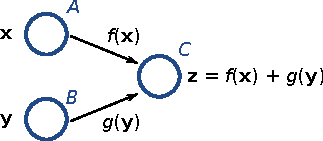
\includegraphics{media/sum_vs_recurrent_a.pdf}
		\caption{Feed forward network}
		\label{fig:feed_forward_recurrent_a}
	\end{subfigure}
	\begin{subfigure}[b]{0.4\textwidth}
		\centering
		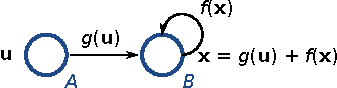
\includegraphics{media/sum_vs_recurrent_b.pdf}
		\caption{Recurrent network}
		\label{fig:feed_forward_recurrent_b}
	\end{subfigure}
	\caption{Comparing a feed-forward and a recurrent neural network.}
	\label{fig:feed_forward_recurrent}
\end{figure}

\Note{When we talk about recurrent connections in the context of the Neural Engineering Framework, we typically refer to a single neuron population that is connected back to itself. While this might seem a little strange, this section is meant to point out that recurrent connections change virtually nothing in terms of the equations that we have used so far.}

\paragraph{Revisiting a neural population receiving input from two pre-populations}
As we discussed in the last lecture, \cref{fig:feed_forward_recurrent_a} depicts an ensemble $C$ receiving input from two pre-ensembles $A$ and $B$. Mathematically, each neuron $i$ in the post-population $C$ receives an input current $J^C_i(t)$
\begin{align*}
	J^C_i(t) &= \big\langle \vec w_i^A , \big ( \vec a^{A}_\mathrm{pre} \ast h \big)(t) \big\rangle
	        + \big\langle \vec w_i^B , \big ( \vec a^{B}_\mathrm{pre} \ast h \big)(t) \big\rangle
	        + J^\mathrm{bias}_i \,,
	       & \text{where } \vec w^A_i = \big( \mat E \mat D^{g_1} \big)_i \text{ and } \vec w^B_i = \big( \mat E \mat D^{g_2} \big)_i \,,
\end{align*}
where $\vec a^{A}_\mathrm{pre}$ and $\vec a^{B}_\mathrm{pre}$ are the activities of the pre-populations $A$, $B$, respectively. The function $h$ is the synaptic filter, $\mat E$ is a matrix of post-population encoders, $\mat D^{g_1}$ is decoding the function $g_1(\vec x)$ from population $A$, $\mat D^{g_2}$ is decoding the function ${g_2}(\vec y)$ from the pre-population population $B$. Then, the value $\vec z$ represented by the population is approximately $\vec z = f(\vec x) + f(\vec y)$.

\paragraph{Recurrent populations}
We can use the same setup as above to implement the recurrent connection depicted in figure \cref{fig:feed_forward_recurrent_b}. Here, a population $B$ represents a value $\vec x$ and receives input from both a pre-population $A$ representing a value $\vec u$, as well as itself -- representing the value $\vec x$. That is, each neuron $i$ in $B$ receives the current
\begin{align*}
	J^B_i(t) &= \big\langle \vec w_i^A , \big ( \vec a^{A}_\mathrm{pre} \ast h \big)(t) \big\rangle
			+ \big\langle \vec w_i^B , \big ( \vec a^{B}_\mathrm{pre} \ast h \big)(t) \big\rangle
			+ J^\mathrm{bias}_i \,,
			& \text{where } \vec w^A_i = \big( \mat E \mat D^{g_1} \big)_i \text{ and } \vec w^B_i = \big( \mat E \mat D^{g_2} \big)_i \,.
\end{align*}
Notice that apart from names, there is virtually no difference between the previous two equations. The population $B$ approximately represents the value $\vec x = g(\vec u) + f(\vec x)$. In terms of control theory, the variable $\vec u$ is the \emph{input} to our system, whereas the variable $\vec x$ is the represented value. The function $g(\vec x)$ is a function transforming our input, the function $f(\vec x)$ is the \emph{feedback function}.

\Note{When implementing a computer simulation that contains recurrent connections, each occurrence of a population pre-activity $\vec a_\mathrm{pre}$ should be interpreted as the pre-population activity from the last timestep.

Note that this will introduce a delay of one timestep each time a new set of populations is connected. While not much of an issue in general, this delay is not part of the continuous equations that are being simulated. The implementation of the Neural Engineering Framework in \emph{Nengo} is thus a little more clever and will only introduce delays if it has to; it will not introduce a delay on pure feed-forward connections.}

\subsection{Experimenting With Recurrent Connections}


\begin{figure}
	\centering
	\begin{subfigure}{\textwidth}
		\centering
		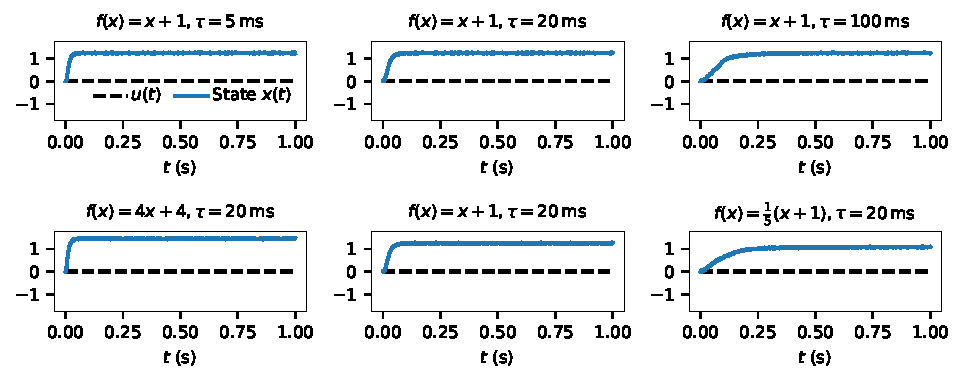
\includegraphics{media/fxp1_example_small.pdf}\\[-0.25cm]
		\caption{Exploring the feedback function $f(\vec x) = x + 1$}
		\label{fig:dynamics_example_a}\vspace{0.25cm}
	\end{subfigure}
	\begin{subfigure}{\textwidth}
		\centering
		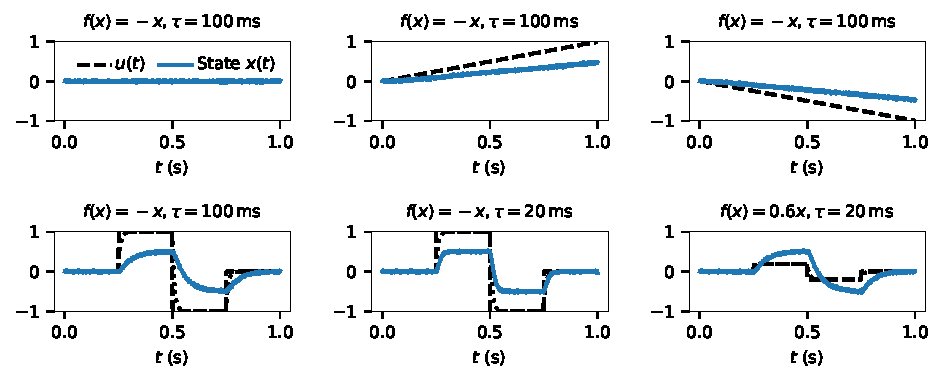
\includegraphics{media/fmx_example_small.pdf}\\[-0.25cm]
		\caption{Exploring the feedback function $f(\vec x) = -x$}
		\label{fig:dynamics_example_b}\vspace{0.25cm}
	\end{subfigure}
	\begin{subfigure}{\textwidth}
		\centering
		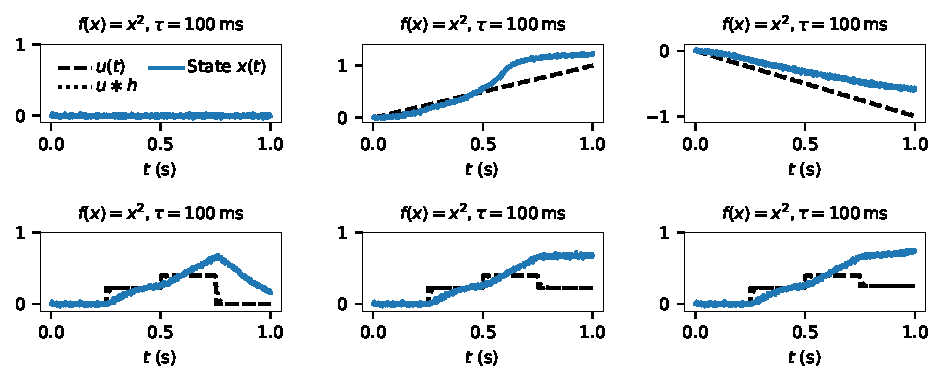
\includegraphics{media/fxs_example_small.pdf}\\[-0.25cm]
		\caption{Exploring the feedback function $f(\vec x) = x^2s$}
		\label{fig:dynamics_example_c}\vspace{0.25cm}
	\end{subfigure}
	\caption{Exploring the effect of different feedback functions $f(\vec x)$, input signals $u(t)$, and synaptic time constants $\tau$ on the dynamics of a single-population network. $100$ LIF neurons, decoded data are filtered with a \SI{10}{\milli\second} time-constant exponential low-pass.  \CodeLink{lecture_06/media/code/dynamics_experiments.ipynb}}
	\label{fig:dynamics_example}
\end{figure}

The above equations illustrate how recurrent connections are implemented and what the represented value of the recurrently connection is. To get some intuition for the dynamics of such a system, we can test different feedback functions $f(\vec x)$. \Cref{fig:dynamics_example} depicts the behaviour of a population of LIF neurons representing a one-dimensional value along with various feedback functions and various synaptic filter time constants.

\Note{The synaptic filter $h(t)$ we are using here is the exponential low pass
\begin{align}
	h(t) &= \begin{cases}
		\frac{1}\tau e^{-t / \tau} & \text{if } t \geq 0 \,,\\
		0 & \text{if } t < 0 \,.\\
	\end{cases}
	\label{eqn:filter}
\end{align}
This a version of the general synaptic filter discussed in lecture four (in particular $n=0$). For this specific case, we can compute the normalisation factor $c$ in closed form. It holds $c = \frac{1}{\tau}$. To see that this factor is correct, we can compute the integral
\begin{align*}
	\int_{0}^\infty h(t) \,\mathrm{d}t &= \int_{0}^\infty \frac{1}\tau e^{-t / \tau} \,\mathrm{d}t = \frac{1}{\tau} \big[  -\tau e^{-t / \tau}  \big]_0^\infty = \frac{1}{\tau} \big[  0 + \tau  \big] = 1 \,.
\end{align*}}

\paragraph{Feedback $f(x) = x + 1$}
The dynamics of the system for a feedback function $f(x) = x + 1$ are depicted in \cref{fig:dynamics_example_a}. The resulting system converges to a value slightly above one. The rate of convergence is determined by the time constant $\tau$ and the scaling of the feedback function; an increase of the time constant by a factor $c$ seems to result in similar dynamics as dividing the feedback function $f$ by $c$.

\Note{This system only converges to a fixed value due to saturation of the neural responses. For example, if we replace the LIF neurons with rectified linear units, the state $x$ will diverge monotonically towards infinity.}

\paragraph{Feedback $f(x) = -x$}
The dynamics of a system with the feedback function $f(x) = -x$ are depicted in \cref{fig:dynamics_example_b}. The system converges to exactly one half of the input $u(t)$. Rearranging the function describing the represented value $x$ yields
\begin{align*}
	x = g(u) + f(x) = u - x \Leftrightarrow x = \frac{u}2 \,.
\end{align*}
This explains why the function converges to a steady state of $\frac{u}2$; however, this analysis does not help us to understand the dynamics of the system (e.g.,~the bottom half of \cref{fig:dynamics_example_b}).

\paragraph{Feedback $f(x) = x^2$}
The dynamics for a feedback function $f(x) = x^2$ are depicted in \cref{fig:dynamics_example_c}. The system converges to $u(t)$ for inputs $u(t) \lessapprox 0.4$ but diverges for larger values. Interestingly, once the system is in a state with $x > 0.4$, it will not converge back to $u(t)$ for values of $u(t)$ between approximately $0.2$ and $0.4$. This means that the system has some kind of memory. For negative inputs $u(t)$ the system approximately converges to $\frac{1}2 u(t)$.

\section*{Mathematical Analysis}

\begin{figure}
	\centering
	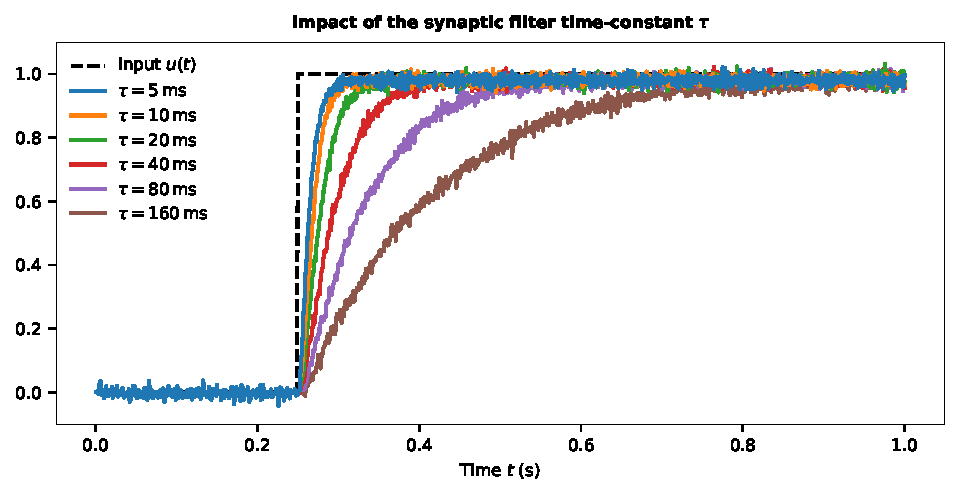
\includegraphics{media/synaptic_filter.pdf}\\[-0.5cm]
	\caption{Dynamics of a feed-forward system for varying synaptic time constants $\tau$. $1000$ LIF neurons, decoded data are filtered with a \SI{1}{\milli\second} time-constant exponential low-pass. \CodeLink{lecture_06/media/code/dynamics_experiments.ipynb}}
	\label{fig:synaptic_filter}
\end{figure}

\Note{While the above examples give us a feeling for what the dynamics of a neural system with recurrent connection might look like, these systems remain quite mysterious. We need to perform some mathematical analysis in order to truly understand these networks.}

In order to gain a better understanding of recurrent dynamics, let's first revisit a simple feed-forward network. \Cref{fig:synaptic_filter} shows a single neuron population with varying synaptic filter time-constants $\tau$. As we can see, the dynamics of the system almost exclusively depend on the filter time constant. Furthermore, as we have already discussed, it does not matter whether we apply the filter before or after the encoding process. Correspondingly, it is sufficient to analyse dynamics in terms of represented values and to ignore individual neurons.

\Note{\emph{Assumptions.} As so often, we will ignore the fact that we are dealing with vectorial quantities in the following subsection and instead assume that $d = 1$. That being said, all equations also hold for higher-dimensional representations.
	
Furthermore, we will assume that the synaptic filter is the same for both the synapses from the pre-populations, as well as the synapses filtering the recurrent connections. Often, we will find that the recurrent connections have a longer time constant than the input connections. However, the equations we derive still work reasonably well.}

\subsection*{Analysing Neural Network Dynamics}

The equation detailing the recurrence relationship $x = g(u) + f(x)$ did not not take time into account and thus does not include the synaptic filter. Assuming that both the input and the recurrent connections are filtered by the same filter (see the assumptions listed above) we get the following dynamical system:
\begin{align*}
	x(t) &= \big( h \ast \big( g(u) + f(x) \big) \big) (t) = \int_{-\infty}^{\infty} h(t') \big( g(u(t - t')) + f(x(t - t')) \big) \mathrm{d}t' \,.
\end{align*}

Unfortunately, and as we have seen in previous lectures, the convolution operator is a little unwieldy. We could eliminate the convolution by switching to the Fourier Domain, however, there is an alternative, more powerful alternative: the Laplace transformation $\mathcal{L}\{f\} = F(s)$.

\Note{The Laplace transformation is a more general version of the Fourier transformation. 
\begin{align*}
	\mathcal{L}\{f\} = F(s) &= \int_{0}^\infty f(t) e^{-st} \,\mathrm{d}t \,,
\end{align*}
where $s$ is a complex-valued parameter $s = \sigma + i \omega$. Notice that the Laplace and Fourier transformation are almost the same if we let $\sigma = 0$; the major remaining difference are the integration boundaries. Since the lower integration boundary of the Laplace transform is zero (instead of $-\infty$ in the case of the Fourier transformation), the Laplace transformation is more suitable for causal systems.

The Laplace and Fourier transformation share many commonalities, including linearity, and the fact that convolution becomes multiplication. Importantly however, it also holds
\begin{align*}
	\mathcal{L}\left\{ \frac{\mathrm{d}f}{\mathrm{d}t} \right\} &= \mathcal{L}\big\{\dot f\big\} = sF(s) \,,
\end{align*}
that is, a time-differental just turns into multiplication with the variable $s$. This makes the Laplace transformation an important tool for dealing with differential equations.}

The Laplace-transform of the first-order exponential low-pass filter in \cref{eqn:filter} becomes:
\begin{align*}
	\mathcal{L}\{h\}
	    &=  \int_{0}^\infty h(t) e^{-st} \,\mathrm{d}t
		 =  \int_{0}^{\infty} \frac{1}{\tau} e^{-t'/\tau} e^{-st'} \mathrm{d}t' 
		 =  \int_{0}^{\infty} \frac{1}{\tau} e^{-t'(1/\tau + s)} \mathrm{d}t' \\
		&=  \left[ -\frac{1}{\tau \left( \frac{1}{\tau} + s \right)} \right]_0^\infty
		 =  \frac{1}{1 + s\tau}
		 =  H(s) \,.
\end{align*}
Hence, we can rewrite the dynamical system we were looking at in the Laplace domain
\begin{align*}
	X(s) &= H(s) \big(G(s) + F(s) \big)
	\Leftrightarrow X(s) (1 + s \tau) = G(s) + F(s)
	\Leftrightarrow s X(s) = \frac{1}{\tau} \big(G(s) + F(s) - X(s)\big) \,.
\end{align*}
Converting back to the time domain we get the following differential equation
\begin{ImportantEqn}{Recurrent connection differential equation}
	\frac{\mathrm{d}}{\mathrm{d}t} x(t) &= \frac{1}{\tau} \big(g(u(t)) + f(x(t)) - x(t) \big) \,.
	\label{eqn:recurrent_dynamics}
\end{ImportantEqn}
\Note{\emph{Canonical dynamical system, phase portraits, and equilibria.} The canonical form of time-independent a dynamical system
\begin{align*}
	\frac{\mathrm{d}}{\mathrm{d}t} \vec x(t) &= \phi(\vec u(t), \vec x(t)) \,
\end{align*}
where $\phi(u, x)$ is an arbitrary function mapping an input $u$ and the state $x$ onto a state differential. We can draw the function $\phi(u, x)$ as a so called \emph{phase portraits} by drawing an arrow corresponding to the state update in an $x$-$u$ coordinate system (\cref{fig:phase_portraits}).

The points where $\phi(u, x) = 0$ are called \emph{equilibria} (singular: equilibrium). An equilibrium can be either \emph{stable}, or \emph{unstable}. Intuitively, an equilibrium is \emph{stable} if a small perturbance causes the system to converge back to the equilibrium. An equilibrium is \emph{unstable}, if small perturbances cause the system to drift away from the equilibrium point.

Mathematically, one can compute whether a point $(\vec x, \vec u)$ is an unstable equilibrium by computing the Jacobi $J$ matrix of $\phi$ at that point and determining whether any of the real components of the eigenvalues of $J$ are positive.}

\begin{figure}
	\centering
	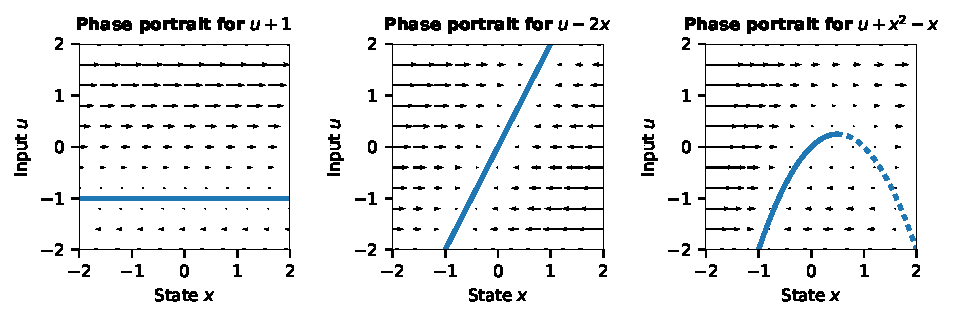
\includegraphics{media/phase_portraits.pdf}
	\caption{Phase portraits (see note) for the dynamical systems corresponding to the three feedback functions we experimented with. Blue lines correspond the equilibria of the dynamical system $f(u, x)$; dotted blue line corresponds to unstable equilibria.  \CodeLink{lecture_06/media/code/phase_portraits.ipynb}}
	\label{fig:phase_portraits}
\end{figure}

\subsection{Analysis of the Previous Experiments}

Given the differential equation in \cref{eqn:recurrent_dynamics} we can now analyse the dynamics of the systems we explored above. Note that in all cases our input translation function $g(u) = u$.

\paragraph{Analysing $f(x) = x + 1$}
For this particular feedback function, our dynamical system becomes
\begin{align*}
	\frac{\mathrm{d}}{\mathrm{d}t} x(t) &= \frac{\mathrm{d}}{\mathrm{d}t} \phi(x(t), u(t)) = \frac{1}{\tau} \big(u(t) + x(t) + 1 - x(t) \big) = \frac{1}{\tau} \big(u(t) + 1 \big) \,.
\end{align*}
Looking at the phase portrait for $f(u, x) = u - 2 x$ in \cref{fig:phase_portraits}, we can see that this function will diverge for inputs $u(t) \neq -1$.

\paragraph{Analysing $f(x) = -x$}
For this feedback function, our dynamical system becomes
\begin{align*}
	\frac{\mathrm{d}}{\mathrm{d}t} x(t) &= \frac{\mathrm{d}}{\mathrm{d}t} \phi(x(t), u(t)) = \frac{1}{\tau} \big(u(t) - 2 x(t) \big) \,,
\end{align*}
which can be re-written as
\begin{align*}
	\frac{\mathrm{d}}{\mathrm{d}t} x(t) &= \frac{\mathrm{d}}{\mathrm{d}t} \phi(x(t), u(t)) = \frac{2}{\tau} \left(\frac{u(t)}{2} - x(t) \right) \,,
\end{align*}
Looking at the phase portrait for $f(u, x) = u - 2x$ in \cref{fig:phase_portraits}, we can see that this system has an line-attractor at $x = \frac{u}{2}$.

\paragraph{Analysing $f(x) = x^2$}
For this feedback function, our dynamical system becomes
\begin{align*}
	\frac{\mathrm{d}}{\mathrm{d}t} x(t) &= \frac{\mathrm{d}}{\mathrm{d}t} \phi(x(t), u(t)) = \frac{1}{\tau} \big(u(t) + x(t)^2 - x(t) \big) \,.	
\end{align*}
This system can be re-written as a dynamical system with two attractors
\begin{align*}
	\frac{\mathrm{d}}{\mathrm{d}t} x(t) &=\frac{1}{\tau} \left( x(t) - 1 + \frac{\sqrt{1 - 4u(t)}}{2} \right) \left( x(t) - 1 - \frac{\sqrt{1 - 4u(t)}}{2} \right) \,.
\end{align*}
These two attractors are visible in the phase portrait for $\phi(u, x) = u + x^2 - x$ (\cref{fig:phase_portraits}); however, we can see that one attractor (on the left side of the portrait) is stable, whereas the other attractor is unstable (right side).

\section{Implementing Arbitrary Dynamical Systems}

\begin{figure}
	\centering%
	\begin{subfigure}{0.5\textwidth}%
		\centering%
		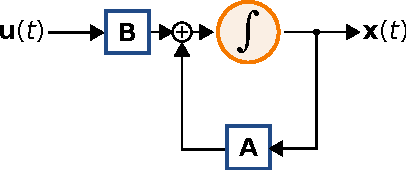
\includegraphics{media/lti_integrator_vs_neural_a.pdf}%
		\caption{Canonical LTI system}%
		\label{fig:lti_integrator_vs_neural_a}%
	\end{subfigure}%
	\begin{subfigure}{0.5\textwidth}%
		\centering%
		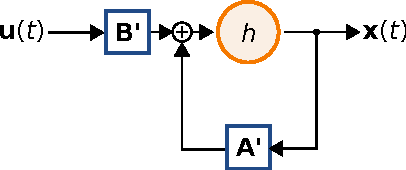
\includegraphics{media/lti_integrator_vs_neural_b.pdf}%
		\caption{Neural LTI system}%
		\label{fig:lti_integrator_vs_neural_b}%
	\end{subfigure}
	\caption{Comparison between an LTI system being evaluated using an integrator, compared to the corresponding neural implementation. Our goal is to find matrices $\mat A'$ and $\mat B'$ such that the two systems are equivalent.}
\end{figure}

We have seen how we can analyse the dynamics emerging from a certain input and feedback function pair $g(\vec u)$, $f(\vec x)$. In other words, given a feedback function $f(\vec x)$ and an input function $g(\vec u)$ we can find the corresponding dynamical system $\phi(\vec u, \vec x)$. This raises the question whether we can also invert this process, i.e.,~given a dynamical system $\phi(\vec u, \vec x)$ find the feedback and input function $f(\vec x)$, $g(\vec u)$ that implement this dynamical system in a neural context.

\subsection{Transforming a Linear Time-Invariant (LTI) System}
We will first look at a special case, a linear time-invariant dynamical system (LTI). This is a dynamical system of the form
\begin{align*}
	\phi(\vec u, \vec x) = \mat A \vec x + \mat B \vec u \,, && \text{ where } \vec u \in \mathbb{R}^{d'}, \vec x \in \mathbb{R}^{d}, \mat A \in \mathbb{R}^{d \times d}, \mat B \in \mathbb{R}^{d' \times d} \,,
\end{align*}
and $\mat A$ is a matrix describing the feedback and $\mat B$ is a matrix describing a mapping from the input onto the state differential.

Normally, we would implement an LTI system using a perfect integrator. Integration of the differential gives us a new state, which is fed back for the computation of the next state differential (\cref{fig:lti_integrator_vs_neural_a}).

However, when building neural networks, we do not have access to a perfect integrator. Instead, we have the synaptic filter $h$, which can be seen as a \enquote{leaky integrator}. Hence, we are looking for a way to rewrite the dynamical system $\phi(\vec u, \vec x)$ into a new dynamical system $\phi'(\vec u, \vec x)$, such that $\phi'$ is equivalent to $\phi$ in the context of a leaky integrator (\cref{fig:lti_integrator_vs_neural_b}). In particular, we would like to find another LTI system
\begin{align*}
	\phi'(\vec u, \vec x) = \mat A' \vec x + \mat B' \vec u \,.
\end{align*}

Writing the canonical dynamical system and the neural dynamical system in the time domain we get
\begin{align*}
	\frac{\mathrm{d}}{\mathrm{d}t} \vec x(t) &= \mat A \vec x(t) + \mat B \vec u(t) \,,&
	\vec x(t) &= \big( h \ast \left( \mat A' \vec x + \mat B' \vec u \right) \big) (t) \,.
\end{align*}
We would like to find $\mat A'$ and $\mat B'$ such that the two systems behave in the same way. Converting to the Laplace to eliminate the convolution we get
\begin{align*}
	sX(s) &= \mat A X(s) + \mat B U(s) \,, &
	X(s) &= H(s) (\mat A' X(s) +  \mat B' U(s))  \,. \\
\end{align*}
Let's expand the right equation and bring it into the same form as the left equation:
\begin{align*}
	X(s) &= \frac{1}{1 + s \tau} (\mat A' X(s) +  \mat B' U(s)) \\
	\Leftrightarrow X(s) (s \tau + 1) &= \mat A' X(s) +  \mat B' U(s) \\
	\Leftrightarrow s \tau X(s) &= \mat A' X(s) +  \mat B' U(s) - X(s)
						    = (\mat A' - \mat I) X(s) + \mat B' \\
	\Leftrightarrow s X(s) &= \frac{1}\tau (\mat A' - \mat I)  X(s) + \frac{1}{\tau} \mat B' \,.
\end{align*}
Comparing to our target equation we get
\begin{align*}
	\mat A &= \frac{1}{\tau} \left( \mat A' - \mat I \right) \,, & \mat B &= \frac{1}{\tau} \mat B' \,.
\end{align*}
Rearranging yields
\begin{ImportantEqn}{Neural implementations of LTI dynamical systems}
\mat A' &= \tau \mat A + \mat I \,, & \mat B' &= \tau \mat B \,.
\label{eqn:nef_lti}
\end{ImportantEqn}


\subsection{Transforming an Additive Time-Invariant System}
We can apply the same math to a non-linear time-invariant dynamical system $\phi$ that can be decomposed into an input translation function $g(\vec u)$ and a feedback function $f(\vec x)$, that is $\phi(\vec u, \vec x) = g(\vec u) + f(\vec x)$. Note that this is more general as a linear time-invariant system -- since $g$ and $f$ can be non-linear functions -- but not quite a general dynamical system.

Assuming that our target system is $\phi '(\vec u, \vec x) = g'(\vec u) + f'(\vec x)$, i.e.,~we would like to find the input translation function $g'$ and the feedback function $f'$ to use in our neural system. Using the same approach as above, we get
\begin{align*}
	X(s) &= H(s) \big(G(U(s)) + F(X(s))\big) \\
	\Leftrightarrow s X(s) &= \frac{1}{\tau} \big( F(X(s)) - X(s) \big) + \frac{1}{\tau} G(X(s))  \,.
\end{align*}
Transforming back to the time domain, comparing to the target system and rearranging yields
\begin{ImportantEqn}{Neural implementation of additive time-invariant dynamical systems}
	f'(\vec x) &= \tau f(\vec x) + \vec x \,,& g'(\vec u) &= \tau \vec u \,.
	\label{eqn:nef_additive_dyn}
\end{ImportantEqn}


\subsection{Transforming Arbitrary Dynamical Systems}

The textbook is also giving an equation that allows us to transform an arbitrary, time-variant dynamical system $\frac{\mathrm{d}x(t)}{\mathrm{d}t} = \phi(\vec u, \vec x, t)$. In this general case we get
\begin{align*}
	\Phi'(U(s), X(s), s) &= \frac{1}{\tau} \Phi(U(s), X(s), s) + X(s) \,.
\end{align*}
As we can see, we generally have to scale our dynamical system by $\frac{1}{\tau}$ and feed back the current state in order to \enquote{remind} the system of its past.

\subsection{Examples}

In this example we are using the above equations in order to implement some common dynamical systems in a neural network.

\paragraph{Integrator}

An integrator is defined as the following dynamical system:
\begin{align*}
	\frac{\mathrm{d} x(t)}{\mathrm{d}t} &= \vec u \,,
\end{align*}
that is, if we write this as a canonical LTI system (\cref{eqn:nef_lti}), we get
\begin{align*}
	\frac{\mathrm{d} x(t)}{\mathrm{d}t} &= \mat A \vec x + \mat B \vec u \,, && \text{where } \mat A = 0, \mat B = \mat I \,.
\end{align*}
Plugging the matrices $\mat A$ and $\mat B$ into \cref{eqn:nef_lti}, we get
\begin{align*}
	\mat A' &= \mat I \,, & \mat B' &= \tau \mat I \,.
\end{align*}
\Cref{fig:example_integrator} shows an integrator implemented in a neural ensemble. In order to verify that our neural implementation is working correctly, we can compute the ideal response.

In particular, for the step function input (left diagram) we get
\begin{align*}
	u(t) &= \begin{cases}
		0 & \text{if } t < 0.1 \,, \\
		1 & \text{if } 0.1 \leq t < 1.1 \,, \\
		0 & \text{if } 1.1 \leq t \,,
		\end{cases} &
	x(t) &= \int_{0}^t u(t') \mathrm{d}t' = \begin{cases}
		0 & \text{if } t < 0.1 \,, \\
		t - 0.1 & \text{if } 0.1 \leq t < 1.1 \,, \\
		1 & \text{if } 1.1 \leq t \,.
	\end{cases}
\end{align*}
We can see that the neural population seems to drift from the ideal value of one, but stays relatively constant afterwards. Such errors are inevitable. Neural implementations of dynamical systems are always approximations. As we have discussed before, errors in neural representations are caused by (at least) two kinds of error: static distortion and noise. Analysing the impact of noise on the dynamics is hard. However, we can analyse this drift by drawing the phase-portraits taking the error due to static distortion into account \cref{fig:example_integrator_phases}.

\begin{figure}
	\centering
	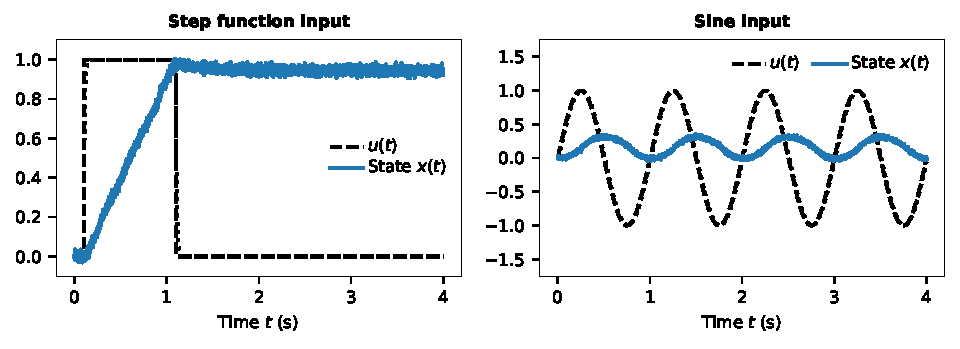
\includegraphics{media/example_integrator.pdf}
	\caption{Dynamics of an integrator implemented using a neural ensemble. Decoded values filtered with a \SI{100}{\milli\second} first-order exponential low pass. The right plot shows the phase portrait of the system implemented by the neural population.  \CodeLink{lecture_06/media/code/nef_implementations.ipynb}}
	\label{fig:example_integrator}
\end{figure}


\begin{figure}
	\centering
	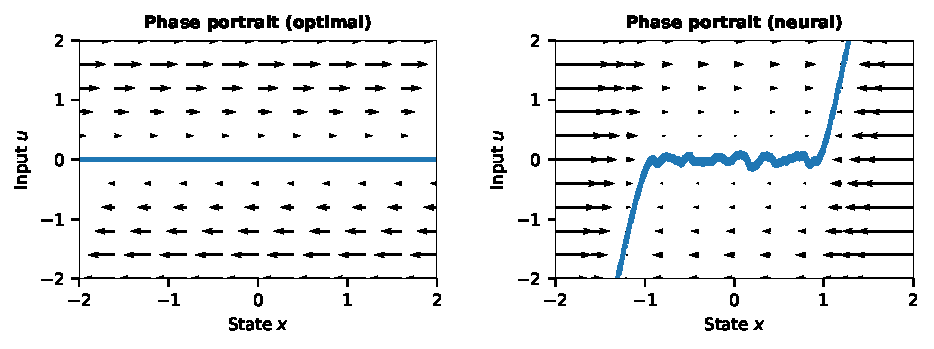
\includegraphics{media/example_integrator_phases.pdf}
	\caption{Phase portraits of the optimal (left) and neural (right) implementation of an integrator. \CodeLink{lecture_06/media/code/nef_implementations.ipynb}}
	\label{fig:example_integrator_phases}
\end{figure}

For the sine wave input (middle diagram) we would expect
\begin{align*}
	u(t) &= \sin(2 \pi t) \,, &
	x(t) &= \int_{0}^t \sin(2 \pi t') \mathrm{d}t' = \left[ -\frac{\cos(2 \pi t')}{2 \pi}  \right]_0^t = \frac{1 - \cos(2 \pi t)}{2 \pi} \,.
\end{align*}
This is also approximately what the neural ensemble is computing.

\paragraph{Oscillator}

\begin{figure}
	\centering
	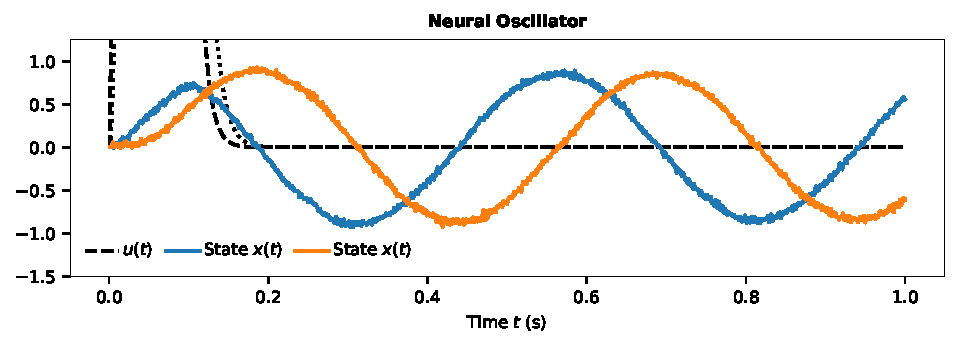
\includegraphics{media/example_oscillator.pdf}
	\caption{Oscillator with $\omega = 4\pi$ (i.e.,~a frequency of \SI{2}{\hertz}). The input in the beginning is required in order to kickstart the oscillator. \CodeLink{lecture_06/media/code/nef_implementations.ipynb}}
	\label{fig:example_oscillator}
\end{figure}

\begin{figure}[t]
	\centering
	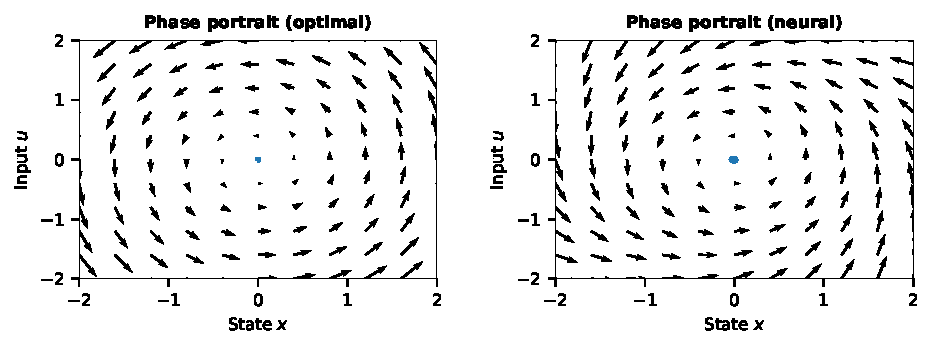
\includegraphics{media/example_oscillator_phases.pdf}
	\caption{Phase portraits of the optimal (left) and neural (right) oscillator dynamics. \CodeLink{lecture_06/media/code/nef_implementations.ipynb}}
	\label{fig:example_oscillator_phases}
\end{figure}

An oscillator can be easily written down in terms of the following LTI system
\begin{align*}
	\mat A &= \begin{pmatrix}0 & -\omega \\ \omega & 0\end{pmatrix} \,, & \mat B &= 0
\end{align*}
where $\omega$ is the angular velocity. Applying \cref{eqn:nef_lti} we get
\begin{align*}
	\mat A' &= \begin{pmatrix}1 & -\tau\omega \\ \tau \omega & 1\end{pmatrix} \,,  & \mat B' &= 0 \,.
\end{align*}
The dynamics of the resulting network are depicted in \cref{fig:example_oscillator}. The phase portrait is shown in \cref{fig:example_oscillator_phases}. Notice how the limited dynamic range of the neurons naturally restricts the maximum amplitude of the oscillation.

\paragraph{Lorentz Attractor}

\begin{figure}[t]
	\centering
	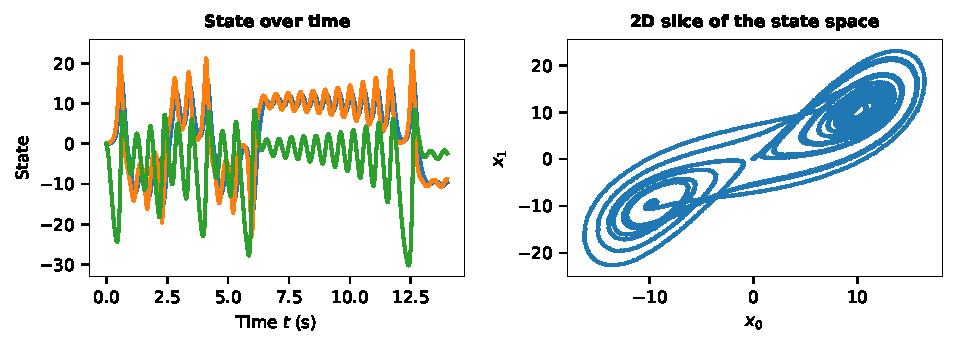
\includegraphics{media/example_lorentz.pdf}
	\caption{Neural implementation of the Lorentz Attractor. \CodeLink{lecture_06/media/code/nef_implementations.ipynb}}
	\label{fig:example_lorentz}
\end{figure}

A variant of the Lorentz Attractor is given as
\begin{align*}
	\frac{\mathrm{d}\vec x(t)}{\mathrm{d}t} &= \begin{pmatrix}
		10 x_2(t)-10x_1(t) \\
		-x_1(t) x_3(t)-x_2(t) \\
		 x_1(t) x_2(t) - \frac{8}{3}(x_3(t)+28)-28
	\end{pmatrix} \,.
\end{align*}
we can use \cref{eqn:nef_additive_dyn} to implement this system as a neural ensemble. An example showing this attractor is given in \cref{fig:example_lorentz}.

%
%\paragraph{Gated Integrator}
%
%\begin{align*}
%	f(\vec x) &= 0 & g(\vec u, \alpha) &= \alpha \vec u \\
%	f'(\vec x) &= \mat I & \Leftrightarrow g'(\vec u, \alpha) &= \tau \alpha \vec u
%\end{align*}
%
%\paragraph{Controlled Oscillator}
%
%\begin{align*}
%	f(\vec x, \alpha) &= \begin{pmatrix}0 & -\alpha\omega \\ \alpha\omega & 0\end{pmatrix} \vec x & g(\vec u) &= 0 \\
%	\Leftrightarrow f'(\vec x, \alpha) &= \begin{pmatrix}1 & -\alpha\tau\omega \\ \alpha\tau \omega & 1\end{pmatrix} \vec x  & \Leftrightarrow g'(\vec u) &= 0
%\end{align*}

\section{Dynamics in Biological Systems: Eye Control}

\begin{figure}
	\centering
	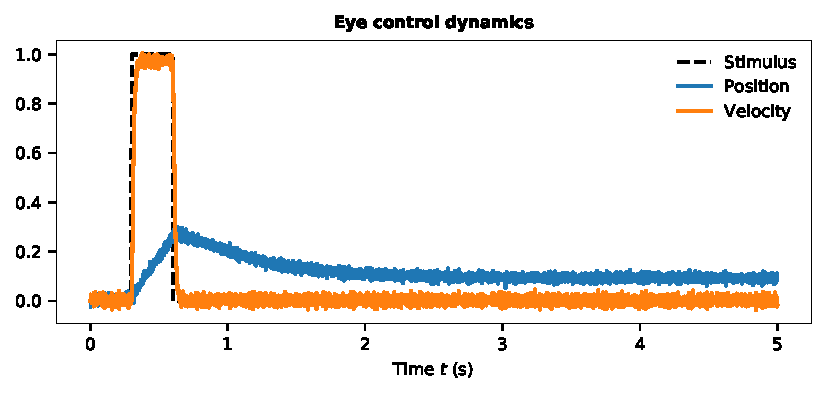
\includegraphics{media/example_eye_control.pdf}
	\caption{Simple horizontal eye control model}
\end{figure}

As an example of a dynamical system in biology, we can have a look at horizontal eye control. We know that horizontal eye position is controlled within a part of the brainstem called \enquote{Nuclei Prepositus Hypoglossi}. In particular, we know that this part of the brain receives an eye velocity $v$ as an input $u(t)$ and outputs an eye position $x(t)$, which in turn is translated into corresponding muscle tensions.

The optimal dynamical system that turns a velocity signal into a position is an integrator. We know from above how to implement a perfect integrator. However, further experiments reveal that the neural circuit in the Nuclei Prepositus Hypoglossi is not a perfect integrator. If a person is told to fixate a point, and we afterwards turn the light off while telling the person to still look into the same direction, their eye will drift back to the centre. This is not due to some mechanical effect in the motor system, but due to the representation produced by the Nuclei Prepositus Hypoglossi converging back to zero. This \enquote{drift to the centre} can be modelled as a leaky integrator with an exponential decay with a time constant $\tau_\mathrm{eye}$ of approximately \SI{70}{\second}.

Correspondingly, we get the following differential equation describing the dynamics of the horizontal eye control system
\begin{align*}
	\dot x(t) &= - \frac{1}{\tau_\mathrm{eye}} x + v \,.
\end{align*}
This is an LTI system. The corresponding NEF model would thus be
\begin{align*}
	\mat A' &= \tau - \frac{1}{\tau_\mathrm{eye}} + 1 \,,´&
	\mat B' &= \tau \,.
\end{align*}

\printbibliography

\end{document}

